\documentclass[../../main.tex]{subfiles}

\begin{document}

\chapter{Establishing a methodology for compile time benchmarking}

With libraries like Eigen\cite{eigen}, Blaze\cite{blazelib}, or CTRE\cite{ctre}
being developed with a large tempalte metaprogrammed implementation, we're seeing
increasing computing needs at compile time. These needs might grow even larger
as \cpp embeds more features over time to support and extend this kind of
practices, like compile time containers\cite{more-constexpr-containers} or static
reflection\cite{static-reflection}. However, there is still no clear cut methodology
to compare the performance impact of different metaprogramming strategies. But
as new \cpp features allow for new techniques with claimed better compile time
performance, no proper methodology is provided to back up those claims.

In this chapter I introduce \ctbench, which is a set of tools for compile time
benchmarking and analysis in \cpp. It aims to provide developer-friendly tools
to declare and run benchmarks, then aggregate, filter out, and plot the data to
analyze it. As such, \ctbench is meant to become the first layer of a proper
scientific methodology for analyzing compile time program behavior.

We'll first have a look at current tools for compile time profiling and
benchmarking and establish the limits of current tooling, then I'll explain
what \ctbench brings to overcome these limits.

\section{Compile time benchmarking: state of the art}

\cpp template metaprogramming raised interest for allowing computing libraries to
offer great performance with a very high level of abstraction. As a tradeoff for
interpreting representations of calculations at runtime, they are represented at
compile time, and transformed directly into their own programs.

As metaprogramming became easier with \cpp11 and \cpp17, it became more mainstream
and consequently, developers have to bear with longer compilation times without
being able to explain them. Therefore, being able to measure compilation times
is increasingly important, and being able to explain them as well. A first
generation of tools aims to tackle this issue with their own specific
methodologies:

\begin{itemize}
\item Buildbench\cite{buildbench} measures compiler execution times for basic
      A-B compile time comparisons in a web browser,
\item Metabench\cite{metabench} instantiates variably sized benchmarks using embedded
      Ruby (ERB) templating and plots compiler execution time, allowing scaling
      analyses of metaprograms,
\item Templight\cite{templight} adds Clang template instantiation inspection
      capabilities with debugging and profiling tools.
\end{itemize}

\subsection{Clang's built-in profiler}

% TODO: More details about time trace JSON structure

Additionally, Clang has a built-in profiler\cite{time-trace} that provides in-depth
time measurements of various compilation steps, which can be enabled by passing
the `-ftime-trace` flag. Its output contains data that can be directly linked to
symbols in the source code, making it easier to study the impact of specific
symbols on various stages of compilation. The output format is a JSON file meant
to be compatible with Chrome's flame graph visualizer, that contains a series of
time events with optional metadata like the mangled \cpp symbol or the file
related to an event. The profiling data can then be visualized using tools such
as Google's Perfetto UI as shown in figure \ref{fig:perfetto-time-trace-ui}.

\begin{figure}[h]
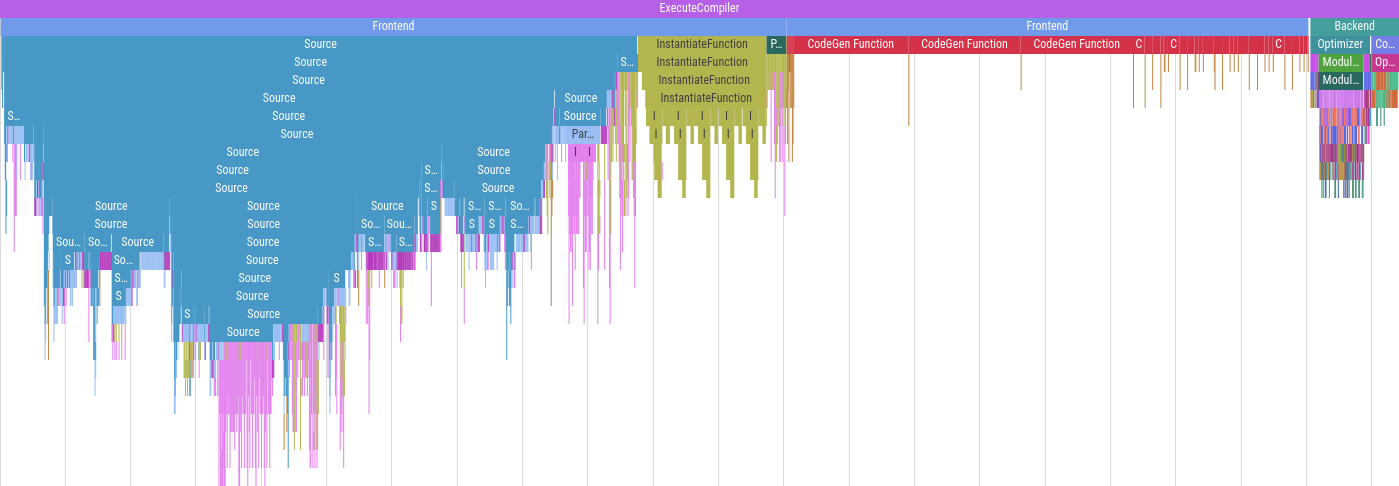
\includegraphics[scale=0.264]{images/perfetto-ui.png}
\caption{Clang time trace file in Perfetto UI}
\label{fig:perfetto-time-trace-ui}
\end{figure}

Clang's profiler data is very exhaustive and insightful, however there is no
tooling to make sense of it in the context of variable size compile time
benchmarks. \ctbench tries to bridge the gap by providing a tool to analyze
this valuable data. It also improves upon existing tools by providing a solution
that's easy to integrate into existing CMake projects, and generates graphs in
various formats that are trivially embeddable in documents like research papers,
web pages, or documentations. Additionally, relying on persistent configuration,
benchmark declaration and description files provides strong guarantees for
benchmark reproductibility, as opposed to web tools or interactive profilers.

\section{ctbench features}

Originally inspired by Metabench\cite{metabench}, \ctbench development was
driven by the need for a similar tool that allows the observation of Clang's
time-trace files to help get a more comprehensive view on the impact of
metaprogramming techniques on compile times. A strong emphasis was put on
developer friendliness, project integration, and component reusability.

\ctbench provides:

\begin{itemize}
\item a well documented CMake API for benchmark declaration, which can be
      generated using the \cpp pre-processor,
\item a set of JSON-configurable plotters with customizable data aggregation
      features and boilerplate code for data handling, which can be reused as a
      \cpp library.
\end{itemize}

In addition to \ctbench's time-trace handling, it has a compatibility mode
for compilers that do not support it like GCC. This mode works by measuring
compiler execution time just like Metabench\cite{metabench} and generating a
time-trace file that contains compiler execution time. Moreover, the tooling
allows setting different compilers per target within a same CMake build,
allowing black-box compiler performance comparisons between GCC and Clang for
example or comparisons between different versions of a compiler.

All these features make \ctbench a very complete toolkit for compile time
benchmarking, making comprehensive benchmark quick and easy, and the only
compile time benchmarking tool that can use Clang profiling data for metaprogram
scaling analysis.

\subsection{CMake API for benchmark declaration}
\label{lbl:ctbench-cmake-api}

The decision of using CMake as a scripting language for \ctbench was rather
straightforward as it is the most widely used build system generator for \cpp
projects.

In this subsection I'll explain the CMake API. It provides functions for
generating benchmark targets at several sizes, and with a specific directory
layout that can be read by the \grapher tools. It also provides functions for
generating graph targets to compare benchmark cases.

\begin{lstlisting}[
  language=cmake,
  caption=ctbench CMake API use example,
  label=lst:ctbench-api-example
]{}
# Fine ctbench package
find_package(ctbench REQUIRED)

# Set benchmark parameters:
# range and number of samples

# From 1 to 10 with a step of 1
set(BENCH_RANGE 1 10 1
  CACHE STRING "Bench range")

# 10 samples per benchmark iteration
set(BENCH_SAMPLES 10
  CACHE STRING "Samples per iteration")

# Add time trace options to enable Clang's
# profiler output, and set the granularity
# to the tiniest value for accurate data
add_compile_options(-ftime-trace -ftime-trace-granularity=1)

# Declare benchmark targets
# with previously defined parameters

ctbench_add_benchmark_for_range(
  hello_world-flat
  hello_world/flat.cpp
  BENCH_RANGE ${BENCH_SAMPLES})

ctbench_add_benchmark_for_range(
  hello_world-pass_by_generator
  hello_world/pass_by_generator.cpp
  BENCH_RANGE ${BENCH_SAMPLES})

# Declare graph target
ctbench_add_graph(
  bfbench-consecutive_loops
  graph-config.json
  hello_world-flat
  hello_world-pass_by_generator)
\end{lstlisting}

Listing \ref{lst:ctbench-api-example} shows how to use the CMake API to generate
a graph comparing two fictional benchmark cases. Each benchmark case is
instantiated at sizes going from 1 to 10 with a step of 1, with 10 samples for
each size. These are defined in the \lstinline{BENCH_RANGE} and
\lstinline{BENCH_SAMPLES} variables, respectively.

The \lstinline{add_compile_options} function is a CMake primitive that allows
setting compile options for the target declarations that follow it. We are using
it to enable Clang's profiler, and set the granularity to its minimum (\ie 1
microsecond) for very fine data gathering.

Then we use the \lstinline{ctbench_add_benchmark_for_range} to declare two
benchmarks targets named \lstinline{hello_world-flat} and
\lstinline{hello_world-pass_by_generator}. The function takes a target name, a
\cpp source file, a range variable name, and a sample number as parameters.
A similar function called \lstinline{ctbench_add_benchmark_for_size_list} allows
defining benchmark targets using a list of sizes instead of an incremental
range.

Both commands will declare CMake targets that generate the time trace files.
The files will be located at the following path:
\lstinline{<benchmark target name>/<iteration size>/<iteration number>.json}.
This
Moreover, the compiler is called through a compiler launcher to work around
CMake's lack for access to compile commands.

At this point we can declare a graph target using \lstinline{ctbench_add_graph}.
It takes a target name and a path to a JSON configuration file followed by an
arbitrary number of benchmark targets as arguments.

\subsection{JSON API for plotter configuration}

JSON configuration files are used to pass parameters such as the plot generator
name, some generic plotting parameters such as an export format list or axis
names, and generator specific parameters like predicates for filtering or group
key specifiers for aggregating time trace events.

\begin{lstlisting}[language=json,
  caption=ctbench configuration file example,
  label=lst:ctbench-config]{}
{
  "plotter": "compare_by",
  "legend_title": "Timings",
  "x_label": "Benchmark size factor",
  "y_label": "Time (microsecond)",
  "draw_average": true,
  "average_error_bars": false,
  "draw_median": false,
  "demangle": false,
  "draw_points": false,
  "width": 1000,
  "height": 400,
  "key_ptrs": ["/name", "/args/detail"],
  "value_ptr": "/dur",
  "plot_file_extensions": [".svg", ".png"],
  "filters": [
    {
      "type": "match",
      "regex_match": false,
      "matcher":
      {
        "name": "ExecuteCompiler"
      }
    }
  ]
}
\end{lstlisting}

Listing \ref{lst:ctbench-config} shows a configuration file for the
\lstinline{compare_by} plotter. The \lstinline{key_ptrs} contains a list of
JSON pointers pointing to the time trace event properties that constitute the
keys to aggregate them. Therefore events will be aggregated by the contents of
the fields at the \lstinline{/name} and \lstinline{/args/detail} fields.
Only the events that match the predicates in the \lstinline{filters} field will
be considered, therefore only the \lstinline{ExecuteCompiler} event will be
observed in that case.

This configuration is a good start for compiler execution benchmarking. The
\lstinline{filters} field can be removed to process all time trace events,
but there can be a lot of events making graph generation very long.

Other options are worth mentioning:

\begin{itemize}
\item Graph customization options such as the width and height of the output
      file, legend title, or axis labels.
\item Plot file extensions, allowing several export formats to be used at once.
\item Allowing median and average to be drawn, as well as single data points,
      or even average error bars.
\item \cpp symbol demangling using LLVM's demangler.
\end{itemize}

Time trace event filtering is done through a predicate engine that will be
further explained in subsection \ref{lbl:grapher-predicate-engine}.

\subsection{ctbench-ttw: ctbench's compiler launcher}
\label{lbl:ctbench-ttw}

CMake abstracts most of the compilation process and makes it impossible to
retrieve derivative files in a reliable way. The object files themselves are
compiled into temporary directories before being relocated to their final
locations.

Because time trace result files are located in the same directory as the object
files and are not moved to the output build directory by CMake, a compiler
launcher named \lstinline{ctbench-ttw} was added to the project.
It can be used to compile benchmark targets by setting the
\lstinline{CXX_COMPILER_LAUNCHER} CMake target property.

The launcher catches the compilation flags to then locate and copy time trace
files generated by Clang which are located in the same directory as the object
file. The name of a time trace file is the same as its binary with its extension
replaced by \lstinline{.json}. An object named \lstinline{main.o} would have its
time trace file generated as \lstinline{main.json} in the same directory.

To use the compiler launcher, one simply adds it to the beginning of a command
along with the desired destination for the time trace file.
For example, when compiling a C++ file using the command
\lstinline{clang++ main.cpp -o main.o -ftime-trace}, you can add
\lstinline{ctbench-ttw /tmp/dest.json} as a prefix:
\lstinline{ctbench-ttw /tmp/dest.json clang++ main.cpp -o main.o -ftime-trace}.
Doing so will launch the compiler, locate \lstinline{main.json} and copy it to
\lstinline{/tmp/dest.json}.

\lstinline{ctbench-ttw} was improved over time to can provide other features
that couldn't be implemented using pure CMake, such as compiler execution time
measurement and allowing the use of different compilers for targets inside a
single CMake project. These two additional features make compiler performance
comparison possible for variable sized compile time benchmarks.

\subsection{grapher}

The \grapher component of \ctbench was developed as a tookit that can be used
through executable tools, and as a C++ library as well.

It contains all the code needed to aggregate Clang's time-trace data generated
by \ctbench benchmark targets, read JSON configuration files for plotters, and
generate plots with different plot generators.

\subsubsection{Library for handling benchmark directory structure}

The most important part of \ctbench's \grapher library is its core types.
They define a hierarchy of elements:

\begin{itemize}
\item Benchmark set, which constitutes a set of different benchmark cases to
      compare.
\item Benchmark case, which represents a benchmark case that will be
      instantiated at several sizes.
\item Benchmark instance, a benchmark case instantiated at a given size.
\item Repetition, a single repetition, run, or sample of a benchmark instance.
\end{itemize}

The type definitions are shown in listing \ref{lst:ctbench-core-types}.

\begin{lstlisting}[language=C++, label=lst:ctbench-core-types]{}
struct benchmark_instance_t {
  unsigned size;
  std::vector<std::filesystem::path> repetitions;
};

struct benchmark_case_t {
  std::string name;
  std::vector<benchmark_instance_t> instances;
};

using benchmark_set_t = std::vector<benchmark_case_t>;
\end{lstlisting}

The \grapher library also provides type aliases for containers or even basic
values to enforce the use of coherent types across the whole codebase. The most
important are \lstinline{json_t} and \lstinline{value_t}, which represent JSON
objects and scalar values extracted from JSON objects respectively (see listing
\ref{lst:ctbench-core-aliases}).

\begin{lstlisting}[language=C++, label=lst:ctbench-core-aliases]{}
using json_t = nlohmann::basic_json<boost::container::flat_map>;
using value_t = unsigned long;
\end{lstlisting}

Boost's \lstinline{flat_map} container is used instead of \lstinline{std::map}
for JSON objects instead as overall performance was measurably better with it.

Most importantly, the \grapher library provides a function to extract benchmark
data from a folder structure as laid out by the benchmark declaration functions
described in \ref{lbl:ctbench-cmake-api}.

\subsubsection{Homogeneous plotter engines and CLI boilerplate}

Besides boilerplate code, \grapher also provides an interface for the addition
of new plotters. This and command line interface boilerplate code make the
addition and implementation of new visualization strategies rather
straightforward.

\paragraph{The plotter interface}

The plotter interface

\begin{lstlisting}[
  language=C++,
  label=lst:ctbench-plotter-base,
  caption=\lstinline{plotter_base_t} type definition]{}
struct plotter_base_t {
  virtual ~plotter_base_t() = default;
  virtual void plot(benchmark_set_t const &bset,
                    std::filesystem::path const &dest,
                    grapher::json_t const &config) const = 0;

  virtual grapher::json_t get_default_config() const = 0;
};

using plotter_t = std::unique_ptr<plotter_base_t>;
\end{lstlisting}

\paragraph{Command line interface}

The \grapher project provides a command line interface for interaction with
users through shell commands, and with the CMake API as well. It provides two
executables that serve as drivers for \grapher plotters:

\begin{itemize}

\item \lstinline{ctbench-grapher-plot}: Main program that generates plots.
      It takes a configuration file and an output folder as options followed by
      several benchmark result folders.
      It is essentially a command line interface over plotters.
      It builds a benchmark set, and passes it to a plotter along with a JSON
      config object and a destination folder.

\item \lstinline{ctbench-grapher-utils}: Auxiliary program currently used to
      obtain default JSON configurations for every plotter. Its functionality
      may be extended in the future.

\end{itemize}

The command line interface is implemented using LLVM's CommandLine 2.0 library.
Both programs can be used without \ctbench's CMake API for reuse in any other
scripting environment as CMake may not always be the best way to generate \cpp
compile time benchmark cases.

For example, Metabench\cite{metabench} uses Embedded Ruby as a source code
generator to instantiate benchmarks at arbitrary sizes. Benchmarks could very
well be generated using other methods such as Python scripting, or even
compiling \cpp sources that have already been pre-processed. Note that a staged
pre-processing method could be implemented using the compiler launcher described
in \ref{lbl:ctbench-ttw}.

\paragraph{Example}

\subsubsection{Time trace event predicate engine}
\label{lbl:grapher-predicate-engine}

% TODO

\subsubsection{Other miscellaneous stuff}

% TODO: Error handling for JSON, statistics, and some other stuff


\section{Statement of interest} % TODO: Rework

\ctbench was first presented at the CPPP 2021 conference\cite{ctbench-cppp21}
which is the main \cpp technical conference in France. It is being used to
benchmark examples from the poacher\cite{poacher} project, which was briefly
presented at the Meeting \cpp 2022\cite{meetingcpp22} technical conference.

\section{Related projects} % TODO: Rework

\begin{itemize}

\item Poacher (https://github.com/jpenuchot/poacher): Experimental constexpr
      parsing and code generation for the integration of arbitrary syntax DSL in
      \cpp20

\item Rule of Cheese (https://github.com/jpenuchot/rule-of-cheese):
      A collection of compile time microbenchmarks to help set better
      \cpp metaprogramming guidelines to improve compile time performance
\end{itemize}

\section{Acknowledgements}

We acknowledge contributions from Philippe Virouleau and Paul Keir for their
insightful suggestions.

\end{document}
